\documentclass{VUMIFPSkursinis}
\usepackage{algorithmicx}
\usepackage{algorithm}
\usepackage{algpseudocode}
\usepackage{amsfonts}
\usepackage{amsmath}
\usepackage{bm}
\usepackage{caption}
\usepackage{color}
\usepackage{float}
\usepackage{graphicx}
\usepackage{enumitem}
\usepackage{listings}
\usepackage{subfig}
\usepackage{array}
\usepackage{wrapfig}
\usepackage{longtable}
\usepackage{eurosym}
\usepackage[hidelinks]{hyperref}
\usepackage{todonotes}
\usepackage[utf8]{inputenc}

\definecolor{dkgreen}{rgb}{0,0.6,0}
\definecolor{gray}{rgb}{0.5,0.5,0.5}
\definecolor{mauve}{rgb}{0.58,0,0.82}

% \lstdefinelanguage{Agda}{%
% language=Haskell
% }

\lstset{
  language=Haskell,
  aboveskip=3mm,
  belowskip=3mm,
  showstringspaces=false,
	columns=flexible,
	deletekeywords=[2]{zero, sum, tail},
	deletekeywords={zero, sum, tail},
  basicstyle={\small\ttfamily},
  numbers=none,
  numberstyle=\tiny\color{gray},
  keywordstyle=\color{blue},
  commentstyle=\color{dkgreen},
  stringstyle=\color{mauve},
  breaklines=true,
  breakatwhitespace=true,
	tabsize=3,
	literate={% replace strings with symbols
	{lambda}{{$\lambda$}}{1}
	{araide}{{$\alpha$}}{1}
},
}

\lstdefinelanguage{GoCust}{%
language=Go,
aboveskip=3mm,
belowskip=3mm,
showstringspaces=false,
columns=flexible,
basicstyle={\small\ttfamily},
numbers=none,
numberstyle=\tiny\color{gray},
keywordstyle=\color{blue},
commentstyle=\color{dkgreen},
stringstyle=\color{mauve},
breaklines=true,
breakatwhitespace=true,
tabsize=3,
deletekeywords={append}
}

% Titulinio aprašas
\university{Vilniaus universitetas}
\faculty{Matematikos ir informatikos fakultetas}
\department{}
\papertype{Projektinis darbas}
\title{Programavimo kalbos su priklausomais tipais transliavimas į Go programavimo kalbą}
\titleineng{Dependently typed programming language translation to Go programming language}
\status{4 kurso studentas}
\author{Justas Tvarijonas}
\supervisor{Partn. Doc. Viačeslav Pozdniakov}
\date{Vilnius – \the\year}

% Nustatymai
% \setmainfont{Palemonas} % Pakeisti teksto šriftą į Palemonas (turi būti įdiegtas sistemoje)
\bibliography{bibliografija}

\begin{document}

\maketitle

\tableofcontents

\sectionnonum{Įvadas}
Programavimas yra instrukcijų davimas kompiuteriui, kuris jas vykdo nepaisant to ar jos yra prasmingos ar ne. Kadangi žmonija tampa vis labiau priklausoma nuo kompiuterių, kurie atsiranda kiekviename mūsų gyvenimo aspekte, tampa vis svarbiau kuo labiau sumažinti klaidų kiekį programiniame kode. Tai bandoma įgyvendinti įvairiais metodais, tokiais, kaip detalus projektavimas ar testų rašymas. Pastarasis yra vienas dažniausiai naudojamų metodų, tačiau testavimas parodo ne klaidų nebuvimą, o tik tai, kad jos yra \cite{UHC}.
\par Tipai programavimo kalbose leidžia programuotojui nurodyti numatytą programos elgseną tipų pavidalu. Tipai ne tik padeda programuotojui rašyti teisingą programą, bet taip pat, kompiuteris gali patikrinti ar sukurta programa veikia taip, kaip buvo užrašyta. Paprasčiausias pavyzdys būtų programa, kuri gavusi sąrašą skaičių, prie kiekvieno elemento prideda vienetą, šios programos tikslas yra priimti sąrašą bei sąrašą gražinti.Tai labai abstraktus apibrėžimas, ką ši programa atlieka, tačiau tai suteikia tam tikrą informaciją apie šios programos veikimą.\par
Priklausomų tipų sistemos \cite{schematicApproach} leidžia tipams būti priklausomais nuo konkrečių reikšmių. Programavimo kalbos \cite{agda_book,idris}, kuriose yra naudojami priklausomi tipai leidžia sukurti tikslesnius tipus, kurie padeda daugiau klaidų aptikti kompiliavimo metu, vietoje to, kad tos pačios klaidos išliktų nepastebėtos iki programos veikimo pradžios. Su tipais, kurie turi daugiau informacijos mes daugiau žinome apie galimus programos parametrus bei rezultatus. Taip pat, priklausomi tipai programavimo kalbose suteikia galimybe rašyti įrodymus.
\par Viena iš programavimo kalbų su priklausomais tipais, kuri yra ir šio darbo objektas, yra Agda. Tai funkcinė programavimo kalba, kurios sintaksė yra panaši į plačiau žinomos funkcinės programavimo kalbos Haskell \cite{haskell} sintaksę. Dabartinė Agda implementacija tipų patikrinimais siekia užtikrinti, kad programos bei įrodymai būtų teisingi. Tuo tarpu Go programavimo kalba \cite{Go} yra greitai kompiliuojama, bet ne taip griežtai tipizuota, taigi atsiranda poreikis tam tikras vietas suprogramuoti su Agda programavimo kalba, verifikuoti jas Agda viduje, bei tada sugeneruoti Go kodą, kurį jau galėtų panaudoti egzituojantis Go kodas.\par Taigi, šio darbo tikslas yra išanalizuoti galimybe generuoti Go programavimo kalbos kodą iš Agda kalbos kodo.
\subsectionnonum{Uždaviniai}
\begin{enumerate}[noitemsep]
  \item Pasirinkti pagrindinius Agda programavimo kalbos konstruktus
  \item Rasti pasirinktų Agda konstruktų atitikmenis Go programavimo kalboje
  \item Pasiūlyti galimą Agda duomenų struktūrų transliavimą į Go duomenų struktūras
  \item Pasiūlyti galimą Agda funkcijų transliavimą į Go funkcijas
\end{enumerate}
\section{Priklausomi tipai}
Priklausomi tipai yra tokie tipai, kurie priklauso nuo tipų reikšmių \cite{depentantTypesAtWork}. Pavyzdžiui galime apibrėžti tipą A\textsubscript{n} - sveikasis skaičius, mažesnis už n. Sakome, kad A\textsubscript{n} priklauso nuo skaičiaus n arba A\textsubscript{n} yra tipų, kurie yra indeksuoti pagal skaičių n, šeima. Parametrizuoti tipai, tokie kaip sąrašas susidedantis iš elementų A paprastai nėra vadinami priklausomais tipais, kadangi šios tipų šeimos yra indeksuojamos kitų tipų, o ne tipų reikšmių, kaip yra su priklausomais tipais \cite{depentantTypesAtWork}.
\subsection{Programavimo kalbos su priklausomais tipais}
Šiuo metu yra sukurta nemažai programavimų kalbų, kurios palaiko priklausomus tipus, dalis jų, pavyzdžiui Coq \cite{coq}, buvo sukurtos kaip vadinamasis įrodymų asistentas, kurių pagalba yra rašomi formalūs įrodymai. Kai kurios kalbos, kurios taip pat yra įvardijamos, kaip įrodymų asistentai, pavyzdžiui Agda \cite{agda_book}, gali būti naudojamos ne tik kaip įrodymų asistentai, bet taip pat ir programinės įrangos kūrimui. Egzistuoja ir atvirščias variantas, kur kalbą yra įvardijama kaip bendrinės paskirties programavimo kalba, tačiau taip pat gali būti naudojama kaip įrodymų asistentas, pavyzdžui Idris \cite{idris}. Šiame poskyryje bus trumpai apžvelgtos kelios iš aukčiau paminėtų programavimo kalbų.
\subsubsection{Idris}
Idris yra grynai funkcinė bendrosios paskirties programavimo kalba su priklausomais tipais, kuri taip pat gali būtų naudojama kaip įrodymų asistentas. Idris yra pakankamai stipriai įtakotas Haskell \cite{haskell}, taigi turi nemažai panašumų su Haskell, ypač sintaksėje bei tipuose, nors Idris turi labiau pažengusią tipų sistema \cite{idris}. Idris gali būtų kompiliuojama į C arba JavaScript kodą.
\subsubsection{Agda}
Agda, yra grynai funkcinė kalba, kuri yra įrodymų asistentas, tačiau gali būti naudojama ir programinės įrangos kūrimui. Pirmoji šios kalbos versija buvo išleista 1999 metais. Dabartinė versija (Agda 2) buvo suprojektuota ir įgyvendinta Gothenburgo universiteto tyrimų inžinieriaus Ulf Norell, tai yra visiškas originalios Agda sistemos pertvarkymas. Kaip ir jos pirmtakai, Agda palaiko indukcinius duomenų tipus, šablonų derinimą (\textit{angl.} pattern matching) bei nutraukimo tikrinimą (\textit{angl.} termination checking) \cite{agda_overview}. Agda nėra universali skaičiavimo požiūriu (ne „Turing complete“). Šiuo metu oficialiai palaikomos 2 kompiliatorių posistemės: MAlonzo skirta transliavimui į Haskell, bei kita posistemė skirta transliavimui į JavaScript \par Kadangi šiame darbe aprašomas Agda kalbos transliavimas, apie šią kalbą bus labiau išsiplėsta kitame skyriuje.
\section{Agda programavimo kalba}
Kaip ir minėta buvusiame skyriuje, Agda yra grynai funkcinė programavimo kalba, kurios pagrindinė paskirtis yra įrodymų asistentas. Agda turi įprastus programavimo konstruktus kaip duomenų tipai, šablonų derinimas, „let“ išraiška, moduliai bei įrašai. Ši programavimo kalba pasižymi sintaksė panašia į Haskell programavimo kalbą.
\subsection{Loginė sistema}
Agda pagrindui buvo pasirinkta Zhaohui Luo vieninga priklausomų tipų teorija (\textit{angl.} unified theory of dependent types, UTT) \cite{agdaInitial}, kuri apjungia Martin-Löf loginę sistemą su tipų visatomis bei Coquand-Huet kuntrukcijų skaičiavimą \cite{schematicApproach}. Galime paminėti keletą sintaksės elementų egzistuojančių šioje loginėje sistemoje:
\begin{itemize}
	\item{ Priklausomas funkcijos tipas
		\begin{lstlisting}
(x : A) -> B
		\end{lstlisting}
		Kur funkcija priima argumentą x, kurio tipas yra A, bei gražina rezultatą, kurio tipas yra B, B tipas gali priklausyti nuo argumento x.
	}
	\item Visatos - tai tokie tipai (žymimi „Set“), kurių elementai yra kiti tipai.
\end{itemize}
Agda loginė sistema yra intuicionistinė, arba dar kitaip vadinama konstruktyvioji. Ši logika remiasi konstruktyviuoju įrodymu, joje teisingi yra tik tie dalykai, kuriuos įmanoma sukonstruoti. Dėl šios priežasties šioje logikoje nėra klasikinėje logikoje naudojamo neįtrauktų vidurių dėsnio (\textit{angl.} law of excluded middle) bet dvigubo neiginio teoremos \cite{intuitionistic}.
\subsection{Sintaksė}
Galime išskirti šiuos Agda programavimo kalbos sintaksinius bruožus:
\begin{itemize}
	\item {Agda programavimo kalboje, priešingai negu didelėje dalyje kitų kalbų (kaip Haskell ar Go), konstruktoriai bei identifikatoriai neturi praktiškai jokių leksinių apribojimų, ko pasekoje, identifikatorius galima pavadinti bet kokiais norimais simboliais, pavyzdžiui, toks duomenų tipas yra visiškai legalus:
	\begin{lstlisting}
data _? (araide  : Set) : Set where
	# : araide  ?
	_C_ : araide  -> araide  ? -> araide  ?
	\end{lstlisting}
	}
	\item Tarpai turi didelę įtaką programos kodui, jie naudojami kaip atskiriamieji simboliai
	\item Yra galimybė apsibrėžti operatorių pirmumą, kokia tvarka jie turi būti vykdomi 
\end{itemize}
\subsection{Numanomi argumentai}
Numanomų argumentų mechanizmas leidžia išmesti tas programos dalis, kurias gali išvesti tipo tikrintuvas. Tarkime turime dvi funkcijas:
\begin{lstlisting}
	f : (x : A) -> B x
	g : {x : A} -> B x
\end{lstlisting}
Skirtumas tarp šių dviejų funkcijų yra skliaustų tipas, g funkcija (su riestiniais skliaustais) priima numanomas argumentus, t.y. pati Agda bandis išsiaiškinti, kokia reikšmė turi būti toje vietoje.
\subsection{Duomenų tipai}
Pagrindinis būdas Agda programavimo kalboje apibrėžti duomenų tipus yra per indukcinius bei indukcinius-rekursinius duomenų tipus, kurie yra panašūs į algebrinius duomenų tipus kitose kalbose (pavyzdžiui Haskell). Natūrialiuosius skaičius būtų galima apirėžti taip:
\begin{lstlisting}
data Nat : Set where
	zero : Nat
	suc : Nat -> Nat
\end{lstlisting}
Iš esmės šis apibrėžimas reiškia, kad turime duomenų tipą Nat, kuris turi du konstruktorius: zero ir suc, zero atspindi natūralųjį skaičių 0, o suc n yra prie n pridėtas 1. Pagal indukcijos principą, jeigu n yra natūralusis skaičius, tai ir n + 1 bus natūralusis skaičius. Tarkime natūralųjį skaičių 3 galėtume atvaizduoti tokia eilute: suc (suc (suc zero)).\par Agda palaiko indukcines šeimas (pagal kurias yra sukurti apibendrinti algebriniai duomenų tipai Haskell programavimo kalboje), šiose šeimose kiekvienas duomenų tipo konstruktorius gali gražinti skirtingą tipą. Kadangi Agda yra su priklausomais tipais, galima abiprėžti vektoriaus tipą, kuris priklauso nuo skaičiaus n:
\begin{lstlisting}
data Vec (A : Set) : Nat -> Set where
	[] : Vec A zero
	_::_ : {n : Nat} -> A -> Vec A n -> Vec A (suc n)
\end{lstlisting}
Šiame apibrėžime „(A : Set)“ yra Vec duomenų tipo elemento parametras. Naujai apibrėžto Vec A tipas yra:
\begin{lstlisting}
Nat -> Set
\end{lstlisting}
Tai reiškia, kad Vec A yra Set šeima, kuri yra indeksuojama pagal natūralųjį skaičių Nat.
\par Pasinaudoję jau aprašytais duomenų tipais, galime sukurti funkciją, kuri iš Vec gražina paskutinį elementą:
\begin{lstlisting}
head : {A : Set}{n : Nat} -> Vec A (suc n) -> A
head (x :: xs) = x
\end{lstlisting}
Šį funkcija priima Vec, kuris yra ne mažesnio ilgio nei 1 (funkcijos aprašyme „suc n“ užtikrina, kad vektoriaus ilgis yra bent 1), bei gražina paskutinį jo elementą. Kadangi vektorius tikrai yra ne tuščias, nėra privaloma tikrinti to varianto, kai jis neturi elementų. Ši funkcija priima sarašą, kurį sudaro bet kokio duomenų tipo elementai, atitinkamai galime susikurti įrašo tipą Zmogus, kuris laiko tam tikrą informaciją apie žmogų, bei perrašyti šią funkciją taip, kad ji veiktų tik su zmogaus tipo sąrašu:
\begin{lstlisting}
record Zmogus : Set where
field
	vardas : String
	amzius : Nat

paskutinisZmogus : {n : Nat} -> Vec Zmogus (suc n) -> Zmogus
paskutinisZmogus (x :: xs) = x	
	\end{lstlisting}
Ši funkcija veiks taip pat, kaip ir aukščiau aprašyta funkcija, tačiau bandant perduoti sąraša su kitokio tipo elementais, bus gauta klaida.	
%  \subsection{Konstruktai}
% Galime išskirti šiuos Agda programavimo kalbos konstruktus:
% \begin{itemize}
% 	\item {„with“ - tai konstruktas, kuris leidžia atliktį šablonų patikrinimus pagal išraiškos rezultatą, šis konstruktas iš esmės prideda papildomą argumentą jau aprašytai funkcijai, pavyzdžiui, žemiau matome funckiją, kuri iš 2 skaičių randa mažesnį:
% 	\item 	\begin{lstlisting}
% 	min : Nat -> Nat -> Nat
% 	min x y with x < y
% 	min x y | true = x
% 	min x y | false = y
% 	\end{lstlisting}
% 	Čia „|“ atskiria originalius argumentus ir argumentą pridėtą su with konstruktu.
% 	}
% 	\item „let“ išraiška - tai konstruktas, kuris leidžia aprašyti apibrėžima funkcijos viduje, šis apibrėžimas negali būti nei rekursiškas, nei aprašytas pagal šablonų tikrinimą
% 	\item „where“ blokai - tai šiek tiek panašus konstruktas į let, tačiau plačiau panaudojami, kadangi jie palaiko šablonų tikrinimus. Didelis skirtumas yra ir jų traktavimas kompiliavimo metu, let yra dalis termo, taigi šių apibrėžimų neliekia atliekant tipų patikrinimus, tuo tarpu where yra dalis apibrėžimų ir jie yra kompiliuojami galutiniame variante.
% \end{itemize}
\subsection{Verifikavimas}
Agda kalboje (kaip ir daugelyje kitų programavimo kalbų su priklausomais tipais) yra galimybė indukcijos bei šablonų derinimo pagalba rašyti įrodymus, tipų pavidalu galima užrašyti skirtingas teoremas. Pavyzdžiui, galime susikurti duomenų tipą, kuris nurodo lygybę, bei funkciją cong, kuri parodo, kad jeigu a ir b yra lygūs, tai juos perdavus į funkciją f, rezultatas taip pat bus lygus:
\begin{lstlisting}
data _==_ {A : Set}(x : A) : A -> Set where
  refl : x == x
cong : { A B : Set} -> {a b : A} -> (f : A -> B) -> a == b -> f a == f b
cong f refl = refl
	\end{lstlisting}
Šioje funkcijoje agda tikrina a ir b kintamuosius, tačiau kadangi jie yra pateikti, kaip numanomi argumentai, jų tikrinime nematome.\par Pasinaudojamę šiuo duomenų tipu bei funkcija, galime įrodyti natūraliųjių skaičių asociatyvumą:
\begin{lstlisting}
associativity : (m n p : Nat) -> ((m + n) + p) == (m + (n + p))
associativity zero n p = refl
associativity (suc m) n p = cong suc (associativity m n p)
\end{lstlisting}
Tai vienas iš būdų, kaip Agda kalboje galima įrodyti natūraliųjų skaičių asociatyvumą, tačiau jų egzistuoja ir daugiau.
\par Šiuose poskyriuose paminėti pagrindiniai, tačiau ne visi Agda programavimo kalbos konstruktai, likę konstruktai turėtų būtų įtraukti į ateityje atliekamus darbus.
\section{Go programavimo kalba}
Go programavimo kalba yra greitai kompiliuojama statiškai tipizuota programavimo kalba, kurios sintaksė yra panaši į supaprastintą C kalbos sintaksę \cite{Go}. Vertas paminėta punktas, kad Go programavimo kalba šiuo metu nepalaiko bendrinių (\textit{angl.} generic) tipų.
\subsection{Sintaksė}
Galime išskirti šiuos Go programavimo kalbos sintaksinius bruožus:
\begin{itemize}
	\item Operacijas galima atskirti naujos eilutės simboliu arba kabliataškiu
	\item Identifikatorių vardai turi parasidėti raide arba apatiniu brūkšniu (\_), po kurių gali sekti skaičiai, raidės arba apatiniai brūkšniai.
	\item Tarpai neturi įtakos programos veikimui, todėl gražus lygiavimas nėra privalomas, kad programa kompiliuotųsi
\end{itemize}
\subsection{Valdymo srauto konstruktai}
Galime išskirti šiuos valdymo srauto konstruktus Go programavimo kalboje:
\begin{itemize}
	\item „if-else“ - Šis konstruktas tikrina sąlyginį teiginį, jeigu jo reikšė yra tiesa, tada vykdomas kodas, kuris yra riestinių skliaustų viduje, jeigu ne, tada vykdomas kodas esantis už jų. Verta paminėti, kad Go kalboje nėra populiaraus šio konstrukto sutrumpinimo su simboliais „?“ ir „:“.
	\item {„switch-case“ - Šis konstruktas yra pakankamai panašus į prieš tai minėtą, tačiau suteikia galimybę patogiau patikrinti daugiau variantų, įprastas „switch-case“ atrodo taip:
	\begin{lstlisting}[language=GoCust]
switch reiksme {
	case reiksme1:
	...
	case reiksme2:
	...
	default:
	...
	}
	\end{lstlisting}
	Su šiuo konstruktu taip pat galima lyginti ne tik paprastas reikšmes bet ir tipus. Šie du konstruktai atitinka Agda kalbos šablonų tikrinimą.
	}
	\item „for“ ir „while“ konstruktai - Go kalboje yra tokie konstruktai kaip „for“ ar „while“, kurie leidžia norimą veiksmą atlikti numatytą kiekį kartų.
\end{itemize}
\subsection{Struktūros}
Go kalboje struktūra (\textit{angl.} struct) yra kintamųjų kolekcija, kuri paprastai apibrėžiama kaip naujas tipas. Jos pagalba galima sugrupuoti duomenis į vieną įrašą, pavyzdžiui galime apsirašyti struktūra, kuri savyje turi žmogaus duomenis:
\begin{lstlisting}[language=GoCust]
type zmogus struct {
	vardas string
	amzius  int
}
\end{lstlisting}
Norint sukurti naują sukurtos struktūros tipo kintamajį tai atliekama užrašius struktūros vardą ir riestiniuose skliaustuose nurodant kintamųjų reikšmes, pavyzdžiui: 
\begin{lstlisting}[language=GoCust]
var zmogus1 zmogus = zmogus{"Justas", 23}
\end{lstlisting}
Taip pat yra galimybė sukurtį tuščią struktūrą, tokios struktūros tipo kintamojo sukūrimas atrodytų taip: 
\begin{lstlisting}
tuscia{}
\end{lstlisting}
\subsection{Sąsajos}
Sąsajos (\textit{angl.} interfaces) yra metodų aprašymų rinkinys, jis apibrėžia, kokius veiksmus gali atlikti tipas:
\begin{lstlisting}[language=GoCust]
type zmogausPaieska interface {
	paskutinisZmogus(zmones []zmogus) zmogus
}
\end{lstlisting}
Kuriant naują metodą galime nurodyti apsirašytą sąsaja kaip to metodo priimamo argumento tipą, tuo atvėju metodo argumentas privalo įgyvendinti tuos metodus kurie yra aprašyti mūsų sukurtoje sąsajoje. Panašiai kaip ir su struktūromis, galima sukurti sąsaja, kuri neturi jokio metodo, tokią sąsają įgyvendina visi tipai, išnaudojant tokią sąsają galima gauti panašų veikimą į bendrinius sudėtinius tipus, bet apie tie bus išsiplėta vėlesniame skyriuje.
\subsection{Funkcijos}
Paminėti apie funkcijų exportinimą
Kuriant Go funkcijas yra privaloma nurodyti kokio tipo argumentus ši funkcija priima, bei kokio tipo reikšmę gražina (jeigu gražina). Pasinaudodami aukščiau aprašyta struktūra bei Go masyvo tipu galime aprašyti alternatyvias funckijas aprašytas Agda skyriuje:
\begin{lstlisting}[language=GoCust]
func head(elementai interface{}) interface{} {
	switch nt := elementai.(type) {
		case []zmogus:
			return nt[len(nt)-1]
		default:
			panic("Nezinomas tipas")
	}
}
func paskutinisZmogus(zmones []zmogus) zmogus {
	return zmones[len(zmones)-1]
}
\end{lstlisting}
Funckija, kuri priima ir gražina zmogus tipo struktūrą yra paprasta, tačiau kadangi Go kalboje nėra bendrinių tipų, negalime aprašyti šios funkcijos nenurodant konkretaus masyvo elementų tipo, nebent jos viduje išrašysime visus tipus, kuriuos ji priima. Taip pat, kadangi funkcija head gražina abstraktų interface{} tipo rezultatą, jį gavus ir norint iš jo gauti vardą, reiktų tą rezultatą dar paversti atgal į tipą zmogus. \par Galime palyginti šias Agda ir Go funkcijas, kurios atlieka tą patį uždavinį:
\begin{itemize}
	\item Agda kalboje parašytos funkcijos užtikrina, kad funkcija nepriims tokios sąrašo, kurio apdoroti negalės, tuo tarpu Go kalboje aprašytai funkcijai galime perduoti tuščią sąrašą, ko pasekoje gautume vykdymo laiko (\textit{angl.} runtime) klaidą.
	\item Agda kalboje naudojant bendrinį tipą priimančia funkciją, jos rezultatas iš karto gaunamas su tuo tipu, kuris buvo paduotas, tuo tarpu Go kalboje jis yra interface tipo, iš kurio jį reikia paversti atgal į norimą tipą.
\end{itemize}
\subsection{Generics in go}
aprašyti generics ir patį proposal
\section{Susiję darbai}
Šiuo metu Agda repositorijoje egzistuoja 2 transliatoriai: 
\begin{itemize}
	\item MAlonzo, kuris Agda programinį kodą paverčia į Haskell, iš kurio jis yra sukompiliuojamas naudojant Glasgov Haskell kompiliatorių (\textit{angl.} Glasgov Haskell Compiler, GHC)
	\item JavaScript, kuris Agda programinį kodą paverčia į JavaScript kodą, šio transliatoriaus pagrindinė paskirtis yra internetinių programų kūrimas \cite{html_agda}
\end{itemize}
Taip pat egzistuoja ir daugiau transliatorių, kurie nėra pridėti prie oficialios Agda repositorijos, tai tokie transliatoriai, kaip Utrecht bei Epic \cite{Utrecht,Epic}. Šie ir aukščiau paminėti transliatoriai bus giliau apžvelgti šiame skyriuje.
\subsection{Haskell programavimo kalbos transliatoriai}
\subsubsection{MAlonzo transliatorius}
Numatytasis ir vienas iš 2 agda transliatorių. Kaip jau ir minėta, jis nukreiptas į Haskell programavimo kalbą, iš kurios naudojant GHC gaunami vykdomieji failai (\textit{angl.} executable files). Tai labiausiai subrendęs transliatorius, jo sugeneruotos programos veikia greičiau, negu vėliau sukurtų transliatorių \cite{Utrecht,Epic}. Vienas minusas, kurį galima išskirti apie šį transliatoriu yra tai, kad norint, kad programa praeitų GHC kompiliatorių, transformuojant kodą MAlonzo posistemė tu panaudoti nesaugius prievartinius tipų vertimus (\textit{angl.} unsafeCoersion, tai metodas Haskell kalboje) prieš kiekvieną funkcijos rezultatą bei argumentą, kas išplečia programos kodą. Taip pat, šie tipų vertimai gali neigiamai įtakoti GHC atliekant į tipus orientuotą optimizaciją.
\subsubsection{Utrecht transliatorius}
Skirtingai negu prieš tai minėtas transliatorius, jis konvertuoja į Utrecht Haskell kopiliatoriaus(\textit{angl.} Utrecht Haskell Compiler, UHC) kodą. UHC Core, skirtingai negu GHC Core yra negriežtas, ko pasekoje šiame kompiliatoriuje nėra būtinybės naudoti nesaugius prievartinius tipų vertimus \cite{Utrecht}.\par Kaip ekperimentinis transliatorius buvo pridėtas prie Agda repozitorijos, tačiau su vėlesnėmis versijomis pašalintas dėl labai didelių priklausomybių nuo kitų bibliotekų.
\subsection{Javascript programavimo kalbos transliatorius}
Vienas iš 2 agda transliatorių esančių oficialioje repositorijoje. Agda kodą transliuoja į netipizuotą lambda skaičiavimą (\textit{angl.} untyped lambda calculus) ir tada transformuoja į ECMASript (dar žinomą kaip JavaScript) \cite{html_agda}. Šis transliatorius buvo sukurtas su intencija, kad būtų galima rašyti internetines aplikacijas su Agda programavimo kalba.
\subsection{Epic programavimo kalbos transliatorius}
Epigram kompiliatorius (\textit{angl.} Epigram Compiler, EPIC) - griežta funkcinė kalba, kuri yra sukurta, tam, kad būtų naudojama kaip posistemė funkcinėms kalboms su priklausomais tipais, norint gauti paleidžiamąjį failą, EPIC yra paverčiama į C programavimo kalbos kodą. Šis transliatorius stipriai įtakojo Utrecht transliatoriaus vystymą \cite{Utrecht}.\par Pagal šiame darbe atliktus metrikų patikrinimus šis transliatorius atsilieka programų veikimo greičiu nuo MAlonzo, tačiau jo sugeneruotas kodas yra mažesnių apimčių. 
\section{Agda transliavimas į Go}
Šiame skyriuje aprašomi egzistuojančių transliatorių bendri bruožai, Agda programavimo kalbos tarpinė reprezentacija bei galimas Agda programavimo kalbos konstruktų transliavimas į Go programavimo kalbos konstruktus. Šis transliavimo aprašymas apima keletą pagrindinių Agda kalbos konstruktų, kiti kalbos kontruktai turėtų būti įtraukti į ateities darbus.
\subsection{Egzituojančių transliatorių panašumai}
Apžvelgus šiuo metu esančius Agda kalbos tranliatorius galima įžvelgti keletą bendrų bruožų:
\begin{itemize}
	\item Visi iš šių transliatorių naudoja išorinę funkcijos sąsają (\textit{angl.} foreign function interface), kurios pagalba galima susieti Agda funkcijas ir duomenų tipus su tos kalbos tipais į kurią yra konvertuojamas Agda kodas.
	\item Visi iš šių transliatorių atlieka daugkartinius žingsius kodą verčiant į kitos kalbos kodą, paprastai Agda kodas pirmiausia yra paverčiamas į vidinę sintaksę iš kurios jis verčiamas į tarpine reprezentacija, kuri yra skirtinga kiekvienam transliatoriui ir tik tada iš tos tarpinės reprezentacijos kodas yra verčiamas arba į taikomos kalbos kodą arba į taikomos kalbos tarpinę reprezentaciją.
	\item Visi iš šių transliatorių taikosi į funkcinę arba lambda skaičiavimo tipo kalbą (pasak A. Jeffrey ECMAScript tarpinė reprezentacija yra netipizuotas lambda skaičiavimas su įrašais \cite{html_agda})
\end{itemize}
\subsection{Agda programavimo kalbos tarpinė reprezentacija}
Kompiliuojant agda failus jie praeina pro kelis žingsius, kol pasiekia reprezentaciją, kuri yra naudojama transformavimui į kitas programavimo kalbas:
\begin{figure}[H]
	\centering
	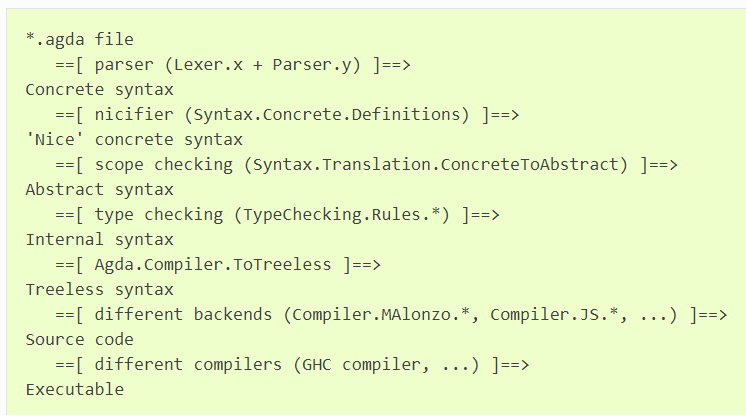
\includegraphics{agdaFileCompilation.png}
	\caption{Žingsiai kol Agda kodas yra paverčiamas kitos kalbos vykdomuoju failu \cite{AgdaWeb}}
	\centering
	\end{figure}
Pagal šį paveikslėlį matome, kad kompiliuojant Agda failą jis praeina pro tokias stadijas: 
\begin{itemize}
	\item Konkreti sintaksė - tai auškto lygio „cukruota“ (\textit{angl.} sugared) sintaksė, ji visiškai atitinka programuotojo įvestą kodą
	\item Abstrakti sintaksė - tai kodo versija prieš tipų patikrinimus, į ją įeina apimties analizė, operatorių pirmenybės išsiaiškinimas. Šioje reprezentacijoje yra atliekami tipų patikrinimai
	\item Vidinė sintaksė - tai paskutinis sintaksės transformavimo etapas prieš atiduodant ją posistemėms. Šiame etape termai yra tinkamai apibrėžti ir tinkamai tipizuoti. Kuriant vidinę sintaksę yra atliekami termų saugumo patikrinimai:
	\begin{itemize}
		\item Funkcijų baigtumo - patikrinama ar rekursiškai aprašytos funkcijos yra baigtinės 
		\item Duomenų tipų pozityvumo - užtikrinama, kad duomenų tipo indukcinio konstruktoriaus aprašyme duomenų tipas nėra kairėje konstruktoriaus tipo pusėje, tai padeda apsisaugoti nuo darbo nebaigiančių funkcijų.
		\item Funkcijų apimties - patikrinama ar šablonų patikrinimas apima visus galimus variantus
	\end{itemize}
	Vidinės sintaksės atvaizdavimui yra naudojamas Haskell duomenų tipas Term.
	\begin{figure}[H]
		\centering
		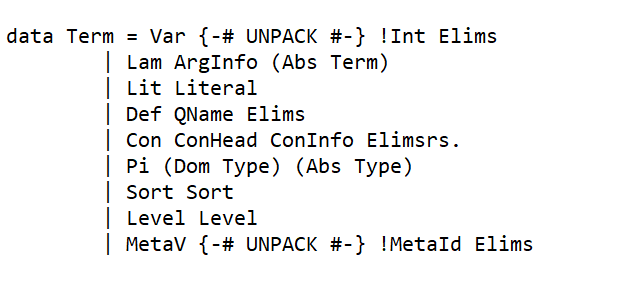
\includegraphics{HaskellTerm.png}
		\caption{Haskell duomenų tipas, kuris yra naudojamas vidinės sintaksės atvaizdavimui}
		\centering
		\end{figure}
		\item Bemedė sintaksė (\textit{angl.} Treeless syntax) - tai sintaksė, kuri skirta kompiliatoriaus posistemei (\textit{angl.} compiler backend) naudoti. Tai yra šiek tiek žemesnio lygio stuktūra negu vidinė sintaksė ir joje nėra atliekami tipų patikrinimai. Šioje sintakėse naudojama atvėjo išraiškos (\textit{angl.} case expressions) vietoje atvėjo medžių (\textit{angl.} case trees), kurie naudojami vidinėje sitaksėje. Šios išraiškos yra Agda funkcijos reprezentacija vidinėje bei bemedėje sintaksėje, iš esmės jos yra panašios, pagrindinis skirtumas yra tas, kad atvėjo išraiškos yra A-normalios formas (\textit{angl.} A-normal-form), tai reiškia, kad kiekvienam patikrinimui yra naudojamas tik vienas kintamasis, kai tuo tarpu atvėjo medžiuose gali būti naudojama ne vienas kintamasis.
\end{itemize}
Tarkime turime paprastą sudėties funkcija Agda kalboje:
\begin{lstlisting}
_+_ : Nat -> Nat -> Nat
zero + m = m
suc n + m = suc (n + m)
\end{lstlisting}
Pavertus į bemedę struktūrą ta pati funkcija atrodo taip:
\begin{lstlisting}
lambda a b ->
	case a of
		demo.Nat.zero -> b
		demo.Nat.suc c -> demo.Nat.suc (demo._+_ c b)
\end{lstlisting}
Čia matome, kad šioje stuktūroje turime atvėjo išraiškas po vieną kintamąjį, šablonų derinimas vyksta nurodant pilną konstruktoriaus vardą (šiuo atvėju „demo“ yra modulio pavadinimas)
\subsection{Agda Duomenų tipų konvertavimas į Go}
konvertavimas į structs ir interfaces. Struktūros kaip list/map naudoja interface{}, todėl casting reiktų po to
\subsection{Agda funkcijų konvertavimas į Go}
\subsubsection{Basic konvertavimas}
.
\subsubsection{builtins}
primitive int type
\subsection{Agda įrašų konvertavimas į Go}
todo iš kodo pusės, bet matyt turėtų pakankamai normaliai verstis į struct, labai panašus formatas
\subsection{Įrodymai}
Galbūt pridėt kažkur atskirai, bet verta paminėt, kad įrodymai yra trinami.
TBD ar iš vis netransliojam, ar turbūt kuriam funkciją, kuri iš kart panic meta.
\subsection{Simbolių užkodavimas verčiant į Go}
Kaip jau buvo minėta ankstesniame skyriuje, Agda leidžia praktiškai bet kokius vardus funkcijoms, bei duomenų tipams, kai tuo tarpu Go kalboje jie yra žymiai labiau ribojami. MAlonzo kompiliatoriuje į Haskell tai apeinama duomenų struktūroms, konstruktoriams, bei funkcijoms įvardinti naudojant naujai sukurtus vardus, pavyzdžiui:
\begin{lstlisting}
name2 = "demo.Nat"
d2 = ()
data T2 = C4 | C6 T2
\end{lstlisting}
kur d2 yra funkcijos vardas, T2 yra duomenų tipo vardas, o name2 yra eilutės tipo kintamasis, kuris saugo funkcijos varda Agda kode. Toks metodas yra tinkamas, kai yra generuojamas vykdomasis failas, bet norint sugeneruoti kodą, kuris yra kviečiamas iš Go kodo toks sprendimas yra netinkamas. Paprasčiausias sprendimas šiam klausimui būtų apriboti simbolius, kuriuos galima naudoti rašant Agda kodą, jeigu yra poreikis jį vėliau kompiliuoti į veikiantį Go kodą. 
\sectionnonum{Rezultatai}
\begin{enumerate}[noitemsep]
  \item Parinkti pagrindiniai Agda programavimo kalbos konstruktai
  \item Surasti pasirinktų Agda konstruktų atitikmenys Go programavimo kalboje
  \item Pasiūlytas galimas Agda duomenų struktūros konvertavimas į Go programavimo kalbą
  \item Pasiūlytas galimas Agda funkcijos konvertavimas į Go programavimo kalbą
\end{enumerate}
\sectionnonum{Išvados}
\begin{enumerate}[noitemsep]
  \item Darbe aprašytus Agda duomenų tipus bei funckijas galima transliuoti į Go sąsajas bei struktūras
  \item Šiuo metu esantys Agda transliatoriai taikosi į funkcines arba labda skaičiavimo kalbas, taigi transliatorius į Go programavimo kalbą būtų pirmasis kompiliuojantis į kitokio tipo kalbą.
\end{enumerate}

\printbibliography[heading=bibintoc] 

\sectionnonum{1 priedas. Agda kodas paverstas į kitas kalbas}
\label{sec:priedas1}
Agda sąrašo tipas ir funkcijos, kurios sudeda sąrašo elementus ir gražina natūralūjį skaičių paverstos į Haskell ir Javascript kalbas. \newline
Haskell:
\begin{lstlisting}
name46 = "demo.List"
d46 a0 = ()
data T46 = C50 | C52 AgdaAny T46	
name36 = "demo.add"
d36 :: Integer -> Integer -> Integer
d36 v0 v1
	= case coe v0 of
			0 -> coe v1
			_ -> let v2 = subInt (coe v0) (coe (1 :: Integer)) in
						coe addInt (coe (1 :: Integer)) (coe d24 (coe v2) (coe v1))
name54 = "demo.sum"
d54 :: T46 -> Integer
d54 v0
	= case coe v0 of
			C50 -> coe (0 :: Integer)
			C52 v1 v2 -> coe d36 (coe v1) (coe d54 (coe v2))
			_ -> MAlonzo.RTE.mazUnreachableError
	\end{lstlisting}
JavaScript:
\begin{lstlisting}
exports["List"] = {};
exports["List"]["empty"] = a => a["empty"]();
exports["List"]["append"] = a => b => c => c["append"](a,b);
exports["add"] = a => b => (
  agdaRTS.uprimIntegerEqual(agdaRTS.primIntegerFromString("0"),a)? b: agdaRTS.uprimIntegerPlus(
    agdaRTS.primIntegerFromString("1"),
    exports["_+_"](
      agdaRTS.uprimIntegerMinus(a,agdaRTS.primIntegerFromString("1"))
    )(b)
  )
  );
exports["sum"] = a => a({
    "append": (b,c) => exports["add"](b)(exports["sum"](c)),
    "empty": () => agdaRTS.primIntegerFromString("0")
  });
	\end{lstlisting}
\end{document}
